% Document template suitable for use as a LaTeX master-file 
% for thesis works in University of Turku Department of Computing
%
% Technical usage guide: https://tech.utugit.fi/soft/thesis/doc/doc/overview/
% 

\documentclass[language=english,version=final,mainfont=none,sharelatex=false]{utuftthesis}
\setcounter{secnumdepth}{2}
\setcounter{tocdepth}{2}
\usepackage{float}
\usepackage[caption=false]{subfig}
\usepackage{lscape}
\usepackage[inkscapelatex=false]{svg}
\usepackage{listings}
\lstset{
    basicstyle=\footnotesize\ttfamily,
    % specifies that lines shouldn't overrun the margin
    breaklines=true
    % specified that, if possible, lines should be broken at whitespace
    breakatwhitespace=true 
}
% Define the algorithm environment
%\makeatletter
\providecommand\textquotedblplain{%
  \bgroup\addfontfeatures{Mapping=}\char34\egroup}
\providecommand{\tabularnewline}{\\}
\floatstyle{ruled}
\newfloat{algorithm}{tbp}{loa}
\providecommand{\algorithmname}{Algoritmi}
\floatname{algorithm}{\protect\algorithmname}
%\makeatother

\addbibresource{Bibliografia.bib}

\begin{document}

\pubyear{2024}
\pubmonth{12}
\publab{Labran nimi?}
\publaben{Laboratory Name}
\pubtype{tkk}
\title{Nix as a declarative and synchronised solution to embedded security challenges and system administration problems for multiple embedded devices}
\author{Eino Korte}

\maketitle
\keywords{tähän, lista, avainsanoista}
% TODO: good/bad keywords

\keywordsen{nix, nixos, declarative, security, pomdp, queries}
\begin{abstract}

Embedded devices are an integral part of our everyday lives; household
machines, automotives, and thermal sensors make use of embedded
devices. They are subject to the global, developing
worlds security problems. This thesis focuses on those found in
public information screens. Embedded devices are particularly
vulnerable to security problems as they have challenges receiving
constant, reliable updates. This thesis' focal point is maintaining,
updating and upgrading embedded devices in a public setting. A
proposed architecture of a public media screen system is provided with example snippets to cover most of common
security issues found in similar setups. The architecture with its
content is then evaluated through with QuERIES methodology. The
central theme of this thesis is Nix, which is a Linux distribution
that forms itself from a set of configuration files, supporting
features like atomic rollbacks and reliable dependency handling. Most
definitive academic sources in this particular subject by Eelco Dostra
are used extensively, as well as papers regarding both embedded
security and measuring security. Ideas for further study are
presented, as security problems may arise in our everyday lives due to
the more mainstream paradigms and could be avoided with the use of
declarative ones.

\end{abstract}

%% \begin{abstraten}
%% Second abstract in english (in case the document main language is not
%% english)
%% \end{abstracten}



% mandatory
\tableofcontents

% if you want a list of figures
\listoffigures

% if you want a list of tables
\listoftables

% if you want a list of acronyms
\listofacronyms

% change the name if the default doesn't sound right
\renewcommand{\algorithmname}{\listingscaption}

% The thesis starts here.

\begin{comment}
To better organize things, create a new tex file for each chapter
and input it below.

Avoid using the å, ä, ö or <space> characters in referred names and
underscores \_ in file names (may break hyperref).

Good luck!
\end{comment}

\chapter{Introduction} \label{johdanto}

A Linux distribution is a bundle of the Linux kernel and a set of
software products called packages \cite{gnuPackagesx2014}. A package
manager is an instrument that handles building packages from either
from source or pre-built binaries, resolving build-time and run-time
dependencies of packages and installing, removing, and upgrading
packages in user environments \cite{gnuPackagesx2014}. Every Linux
device must handle its installed programs with their dependencies and
configurations either imperatively or declaratively. Overwhelmingly
large portion of Linux distributions fall in to the first category
\cite{dolstra2008nixos}. Both imperative and declarative distributions
have their strengths and weaknesses from administrative and security
standpoints.

An imperative distribution provides updatability and modification through a
destructive instrument. Popular imperative package managers are apt,
apk, dnf and zypper \cite{dolstra2008nixos}. Imperative package
managers can remove and overwrite existing files which leaves the
system in an inconsistent state. Different installs have by nature
different states which causes many problems discussed in this
thesis. As files are cross-modified through packages with package
managers such as apt, upgrading can be disastrous as such distributions
don't support atomic rollback capabilities \footnote{Some Linux
distributions using btrfs filesystem can perform a snapshot and
rollback \cite{opensuseSystemRecovery}}. Due to the unpredictability,
often the result can be a partially or completely broken system
\cite{dolstra2008nixos}.

The reference imperative Linux distribution in this thesis is Debian
with its default package manager apt, due to it's popularity and
relative simplicity. The reference declarative distribution is NixOS
with it's partial namesake package manager Nix which provides
declarative configuration of the whole system including the Linux
kernel\footnote{There exists an experimental project that has
succeeded with BSD interoperability
\cite{githubGitHubNixosbsdnixbsd}}. Nix is configured by the Nix
programming language which is inspired by purely functional languages
such as Haskell. \cite{van2013reference}

The reference architecture depicted in chapter \ref{architecture} is
based on Nix as it is the most popular purely functional, declarative
Linux distribution with over 100 000 packages
\cite{nixosNixOSSearch}. Architecture in this context refers to the
set containing clients and server and the used hardware. The term
system means the implementation of the architecture, especially
referred in chapter \ref{analysis}. Depending on the context, system
can also mean a set of procedures, e.g a Linux system. For the term
Linux distribution usually only the word distribution is used.

Another good distribution for the architecture would have been Guix, which has over
28 000 packages \cite{gnuPackagesx2014}. Guix has some improvements
over Nix, including richer and more extensible programming environment
with a Lisp-dialect configuration language, Scheme
\cite{courtes2021deploiements}. NixOS remains as the distribution of
choice, as the number of packages is greater, and general support is
found to be better.

This thesis focuses on the systems and information security of a
reference architecture created with NixOS. Chapter \ref{architecture}
goes through a reference architecture of a solution that handles the
most critical functionalities of an architecture designed for image displaying.

This thesis discusses how declarative distributions can be used as an
improvement over imperative distributions. In chapter \ref{imperative} both approaches to package
management is compared, which is followed by an introduction to
embedded security in chapter \ref{securitystandpoints}. In chapters
\ref{architecture} and \ref{analysis} a quantitative research is
carried out revealing strengths and weaknesses of the reference Nix
environment setup. The selected methodology, QuERIES provide
quantitative results which can be used to improve the security of
declarative architectures. Propositions for further research are
gone through in chapter \ref{further} and finally, chapter
\ref{conclusion} concludes the thesis.

\section{Research methodologies and questions}

Research methodologies used in this thesis are:
\begin{enumerate}
\item a literature review of central papers on subject themes found
  with prepared search statements
\item an action research using a laboratory setup
\item a quantitative research process using QuERIES methodology
\end{enumerate}

Literature review will be addressed mostly in the next section and in
chapter \ref{embedded}. As this thesis' main research methodology is
quantitative, the gathered data points will be addressed as variables
that are compared with mathematical methods. Quantitative methods are
broken down in chapter \ref{securitystandpoints} and
\ref{analysis}. The central methodology is derived from QuERIES, and
the information security aspect is investigated with CIA-triad. In
chapter \ref{analysis} section \ref{whyqueries} QuERIES is compared
with other metrics which are explained in subsection \ref{resquest}.

Quantitative methodologies are oftentimes used in conjunction with
qualitative methodologies, both approaches having their strengths and
weaknesses. One drawback of using qualitative methods in security
framework is their inherent subjectivity. For example the Delphi
technique, where a set of opinions is gathered and compared from a
working group provides subjective substance for a study instead of
objective perspectives \cite{wang2005information}.

The study design in this thesis is \textit{state based}, which refers
to the fact that the research methods focus on different state
transitions, e.g how probable it's for an intruder to gain from
partial leverage to a full control of the system. Qualitative research
wouldn't alone satisfy the requirements, as investigating different
state transitions without quantitative methodologies would be absurd
\cite{ramos2017model}.

\subsection{Literature review}\label{litrev}

This thesis has bibliography from 49 sources, most of it gathered with
a carefully prepared search statement. Other sources include manuals,
material for research methods and other relevant material. The search
statements results presented in next subsection, provide good base
for action research and analysis.

The literature focuses on four main concepts: embedded systems
security with and without declarative components, imperative systems,
measuring security and Nix. The main goal is to find literature that
combines these concepts to gain platform for comparing different
approaches to support the action research.

Central literature revolves around Nix and multiple texts by Eelco
Dostra are cited for illustrating the nuances of a Nix
ecosystem. Other declarative approaches are discussed, by Endres
et. al and Van der Burg \cite{van2010declarative,
  endres2017declarative}. These approaches also contains comparison to
imperative systems, which is the central approach in chapter
\ref{imperative}. Combining cyber security with declarative approaches
were discussed by Specht et. al and Kandoi and Artke
\cite{specht2007analysis, kandoi2021operating}.

Discussion from Ravi et. al and Fysarakis et. al on embedded security
is discussed by \cite{ravi2004security, fysarakis2014embedded}. The
concepts, however are generally too broad for this thesis' scope, so
only the most fitting approaches were selected for use.

The most important literature to measure the security of a system is
by Carin et al. and Hughes and Cybenko \cite{carin2008cybersecurity,
  hughes2013quantitative}. The topics from these papers revolve around
QuERIES, an original approach for measurably improve security. 

\subsubsection{Search statement} \label{searchstatement}

The main search statement for this thesis is: "embedded linux" OR
''declarative'' AND (linux OR *nix) OR deployment OR ''system update''
OR (compare* AND declarative AND imperative AND system*) OR security.

The search statement was prepared to provide as relevant results as
possible for this thesis. The main goal was to include the hypernyms
''embedded linux'', ''linux'' with other terms separated using the
"OR" operator. The subterm (compare* AND declarative AND imperative
AND system*) was chosen to broaden the search to include articles
which compare declarative and interactive systems.

As security is a central theme in this thesis, the term "security" was
included. Search was done on Google Scholar, and other useful material
was handpicked, such as Nix manuals and wiki pages. Systems security
and cyber security material is also included in the bibliography using
search statement ''systems security OR cyber security''. Separate search
''cia-triad'' and ''partial observable Markov chain'' AND
''cybersecurity'' were used to provide tangible meters for measuring
cyber security. To further back up the research for comparing
different metrics, term ''cyber security metric methodology'' was
searched.

For searching specific material about embedded systems, the search
statement ''embedded AND security'' was used. As the need for embedded
toolchains was needed, statement ''yocto AND buildroot'' was
searched. All searches were done on Google Scholar platform.

\subsection{Research questions} \label{resquest}

The research questions for this thesis are:

\begin{enumerate}
\item How can a declarative system be used to measurably improve the
  security of an embedded system used for displaying public media?
\item What are the advantages and/or disadvantages of such system from
  a system administrator standpoint?
\item How can a declarative system be updated from different Linux
  distribution securely and seamlessly?
\end{enumerate}

Research question 1 is the most important and it traverses through
themes of the whole thesis. The hypothesis is that traditional
imperative embedded device fleets have problems which can be solved
with the use of modern declarative systems. First, we aim to gain
information from a specific scenario, presented in chapter
\ref{architecture}, then in chapter \ref{analysis} the gained
information is analyzed and generalized as suitably as possible.

Research question 2 brings up the human element; how can a system
administrator use a new palette of features adequately to provide more
secure system and research question 3 handles a situation where
existing system should be replaced with a NixOS system. How this could
be done securely without risks and preferably easily with existing
tooling is answered in chapter \ref{architecture} section
\ref{instnewdevices}. The next chapter compares imperative approaches
to declarative approaches and provides insight for understanding the
central differences, the emphasis being on how declarative systems can be
used to solve problems better than with imperative systems.

\subsection{Data collection and analysis}

Data collection is done with simulated red–blue team setup, where
either team has a time frame where they must conduct a series of
tasks. These tasks are formalized as partially observable Markov chain
parameters, and analysed with QuERIES methodology. This methodology is
used to gain knowledge and make the system more reliant and better
with multiple iterations. Chapter \ref{analysis} answers research
question 1 and 2 and provides analysis for the reference
system. Research question 3 is answered in chapter \ref{architecture}
section \ref{instnewdevices}.
\input{research.tex}\chapter{Declarative vs. Imperative systems} \label{imperative}

There have been different approaches to declarative modeling of
systems design. Endres et al. compares declarative and imperative
systems from a cloud computing standpoint, and collects systematic
information on what are the strengths and weaknesses of TOSCA, IBM
Bluemix, Chef, Juju, and OpenTOSCA \cite{endres2017declarative}. Van
der Burg and Eelco Dostra use NixOS as a solution for declaratively
distributing into cloud and executing integration and system tests
\cite{van2010declarative}. Most approaches researched through
literature review focus on distributing to cloud, and distributing to
embedded clearly remains as a niche.

Breitenbücher et al. focus on deploying into embedded and discusses
the challenges an IoT user face when deploying a system. It's proven
that setting up devices with mandatory scripts and other actions is a
challenging task, when a number of devices should be set up. Cloud is
something that is useful to be used in tandem with IoT but this thesis
focuses on an \textit{in-premises} reference
solution. \cite{breitenbucher2017declarative}

In this chapter, we focus on comparing different declarative
approaches to the more traditional imperative models, highlighting the
strengths and weaknesses of both. Specifically, examples are provided
to illustrate the limitations often observed in imperative systems,
particularly in terms of reproducibility, scalability and
administration standpoints. Cloud-oriented approaches serve as a prime
reference point for how declarative systems can be effectively
distributed and automated. I argue that similiar approaches as those
taken in cloud should be taken in embedded and IoT to increase security.

\section{Imperative systems}

Imperative deployment models base their functionalities through a
process in which the order of events have a critical significance to
the output \cite{breitenbucher2017declarative}. In context of
virtualization, imperative tooling can be used to form a all
activities to be executed, the control flow, their execution order,
and the data flow between them \cite{endres2017declarative}. This kind
of process is best to be used in conjunction with a formalized
workflow or standard such as BPEL \cite{endres2017declarative}. In
contrast, declarative models don't have such specific requirements, as
these models formalize the processes in the configuration files
\cite{endres2017declarative}.

An imperative system provides updatability and modification through a
destructive instrument. Popular imperative package managers, e.g can
remove and overwrite existing files, which leaves the system in an
inconsistent state \cite{dolstra2008nixos}. Different installs have by
nature different states, which causes many problems discussed in this
thesis.

Imperative systems, while popular, have inherent problems regarding
administrative traits contributing to a framework where the underlying
system has \textbf{no traceability}: the implication that
reproducibility is impossible, as changes to a system are not
traced. Nix provides a solution for this problem with its Nix
generation system. The second point contributes to the fact that with
imperative systems, upgrading is more error-prone than installing from
scratch. This is due to the fact that imperative systems have
\textbf{unpredictable} state, from where the system should migrate to
a predictable state. This causes major issues regarding
upgradability. \cite{dolstra2007purely}

\textbf{The inability to run multiple configurations side-by-side} is
an inherent side effect of a \textit{stateful} system. Declarative
systems don't have this problem: an arbitrary number of configurations
can exist side by side, as the system is defined only by the
configuration, not with the state as a
component. \cite{dolstra2007purely}

\subsection{Debian/Apt}

An example of imperative systems' problematic nature is provided with
the following demonstration. Executing shell command
\begin{lstlisting}
    apt install emacs
\end{lstlisting}
installs a text editor wrapped as a Linux package.  The package emacs
has a dependency, emacs-gtk, which can be removed with command
\begin{lstlisting}
    apt remove emacs-gtk
\end{lstlisting}
Another dependency, emacs-lucid can be removed with command
\begin{lstlisting}
    apt remove emacs-lucid
\end{lstlisting}

we can see that after removing, apt automatically installs emacs-gtk
to avoid breaking the application. The package manager warns:
"emacs-lucid has dependency problems, but removing anyway as you
requested" as shown in figure \ref{deb_remove}. It's also noteworthy,
that the manual page for apt, doesn't say anything about a possible
installation side-effect of a package removal command
\cite{ubuntuUbuntuManpage}.  We could forcibly remove the package by
invoking
\begin{figure}[H]\label{dpkgsnippet}
\begin{lstlisting} 
    dpkg --remove --force-depends emacs-lucid
\end{lstlisting}
\end{figure}
% kuva distribuutioiden distribuutioista
\begin{figure}\label{deb_remove}
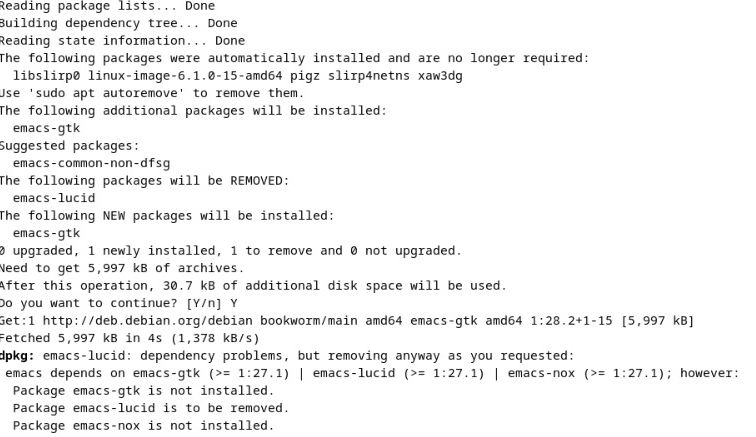
\includegraphics[scale=2.0]{latex/kuvat/cropped_apt_output.jpg}
\label{Terminal output from a Debian system when installing an Emacs package.}
\end{figure}
thus leaving the system in an unreliable state. Dpkg is a low-level
tool associated with apt, and doesn't automatically handle dependency
resolutions or further package relations
\cite{thiruvathukal2004gentoo}. What happens if we had a large number
of devices, in-premises or cloud where all system commands are done
imperatively? We would have a large number of devices that differ from
each other, because as shown, the order of commands affect the state
of the system and the other way around. Time is also a factor that
causes systems to diverge, as packages are not up-to-date by
default. Invoking \begin{lstlisting} apt update
\end{lstlisting}
updates the local repositories to match the download mirrors. If by
technical reasons or possible user error this command is conducted in
the wrong order there will be divergent systems.

Implementing a deployment model with only Debian would be a gruesome
task, as the order of events which occur during the setup phase is
critical. As presented by Endres et al. a formalized workflow graph
would be needed to set up a reliable system. However, a Debian could
be used as a host to user-space application deployment, such as
Bluemix or Chef, where common DevOps practices can be used
\cite{endres2017declarative}.

\subsection{Gentoo/Portage} \label{gentoo}

Gentoo Linux is bundled with the package manager Portage, which
consists of two components: ebuild and emerge, which have similar
relation as dpkg and apt. Portage is primarily source-based package
manager; ebuild builds and installs packages from source and emerge
resolves dependencies and handles other related issues. Portage's
flagship feature is its ''USE-flags'', a mechanism that enables
compiling source files with or without specific features. For example,
a make.conf file in /etc/portage could have USE-flags specified as:
\begin{figure}[H] \label {gentoosnippet1}
\begin{lstlisting}
USE=''-X wayland''
\end{lstlisting}
\end{figure}
and the sources wouldn't, if possible, compile with X11 support, but
would with Wayland. This results in smaller binary sizes, increased
performance and enhanced security through package minimalism. When
there's less dependencies and installed programs, there's also less
attack surface \cite{wang2017network}.

Gentoo's portage system allows sharing binaries and sources with
rsync, which would be a useful feature in a server-client model,
similar to architecture proposed in chapter \ref{architecture}, where updates are centralised
\cite{thiruvathukal2004gentoo}. An architecture with imperative
components isn't proposed in this thesis, but if it would be, a
suitable candidate would be something that uses Gentoo Linux as it's
foundation.

One benefit from Nix is its lightweight tendency to enable system
tests. Integrating system tests with a Gentoo system would require a
considerable amount of work, as setting up such system needs a lot of
configuration and executing commands in a correct order
\cite{van2010automating}. Gentoo definitely fits in an imperative
deployment strategy but the requirement for explicit detail of every
step would be error prone even for a seasoned administrator
\cite{breitenbucher2017declarative}.

\section{Declarative systems} \label{declarativesystems}

Presented problems in chapter \ref{imperative} can be solved using
package manager that is reproducible, reliable and atomic. Package
installs in Nix are in isolation from each other so that they don't
have conflicting effects. This results packages being predictable and
assures they work coherently even if underlying install is
different. Because the packages are declared in a single set of
configuration files it's trivial to reproduce the system in a
different environment. The demonstrated effect in snippet
\ref{dpkgsnippet} was a problem due to lack of isolation. When
dependencies are scattered in the system instead of declared
explicitly in a installed package, a faulty state could be
achieved. Nix assures, that these kind of problems are out of the
question. A result of this is that in a Nix system installs of same
program can reside side-by-side with varying versions
\cite{dolstra2008nixos}.

As presented by Endres et al, systems can be declared, even if the
underlying infrastructure is imperative by nature
\cite{endres2017declarative}. This thesis focuses on purely functional
methodologies which fix the most prevalent issues compared with
imperative models. Tools such as Chef focus on deploying on a
imperative system, which causes an inherent problem with cohesion in a
system that should work regardless of the underlying machine or
network. Alternative deployment tools are discussed in section
\ref{nondeclarative}.

It's also noteworthy that many imperative package mangers don't
support rollback mechanisms. If the Nix configuration file is changed
and the system is rebuilt with command
\begin{lstlisting}
nixos-rebuild switch
\end{lstlisting}
the previous state could be recovered by \begin{lstlisting} nix
  profile rollback
\end{lstlisting}
This is an important feature as the Nix configuration files control
the whole system, they can also leave the system in an undesired
state. Nix switches between \textit{profiles}, which is a way to
provide different configurations for different user environments as
shown in figure \ref{userenvs} and provide atomic upgrades and
rollbacks. \cite{nixosNixOSManual}

\begin{figure}[t!]
\centerline{\includesvg[width=1.0\columnwidth]{latex/kuvat/symlinks.drawio.svg}}
\caption{Relations between different user environments and installed
  programs \cite{nixosUserEnvironment}.}
\label{userenvs}
\end{figure}

A fundamental component of the ecosystem is Nix, a domain-specific
language designed for configurations, distinguished by its functional
nature and lazy evaluation. The concept of purity is central to Nix,
where values remain unchanged throughout computation, and every
function consistently yields the same output regardless of input
\cite{dolstra2013charon}. The security implications of using Nix
vs. an imperative system is discussed in chapter \ref{embedded}.

\subsection{Non-declarative components} \label{nondeclarative}

Declarative distributions such as Nix can't do everything in the
system in stateless manner. Some components of the system, such as
databases must have a distinct state, which can't be practically
declared with package manager apart from initial configurations
\cite{van2013reference}. Home directories can vary as much as the
system administrator desires. For example, a configuration file for
text editor vim is usually declared in the file
/home/<user>/.vimrc. Nix provides multiple ways to perform the whole
configuration process from the Nix configuration files. One way is
declaring the desired .vimrc in the Nix configuration, as in the
following snippet:

\begin{lstlisting}
{
  environment.systemPackages = [
    (pkgs.vimConfigurable.customize {
      vimrcConfig.customRC = ''
        " arbitrary vim config
      '';
    })
  ];
}
\end{lstlisting}
Nix provides also provides ways to fetch content to the system from
remote URLs, and if the administrator doesn't want the system to
remain ''pure'', they can build the system by \begin{lstlisting}
  nixos-rebuild switch --impure
\end{lstlisting}
This results the system having mutable components, which can be
desirable from an accessibility point of view, but can result in
unpredictable behaviour if the impure components are modified. In this
context this means, that the built pure components are read-only and
immutable \cite{dolstra2010nixos}.

User environments (Nix profiles) can be used so that for different
needs, or for different users there are multiple environments in which
the user can operate as shown in figure \ref{userenvs}. User
environments are a successor to the concept, where installed programs
either reside in /usr/bin, /usr/sbin etc. or have a symbolic link to
the said directories. They can be figured as trees of symbolic links
that reside also in the Nix store hence referred packages are called
''activated packages''. Remember, that the traditional Unix directory
structure, where files are separated to /bin/ /sbin/ etc. doesn't
completely apply. Instead, the installed programs reside usually in
/nix/store. \cite{dolstra2008nixos}

There are continuous build and integration services, such as Hydra,
which include Nix-compatible support for handling runtime
configuration and tools, such as Disnix and Charon \footnote{Charon is
now called NixOps \cite{githubNixNixpkgsNixOS}}, which focus on
setting up complementary infrastructure. Van Der Burg presents these
new tools to replace Cfengine, Puppet and Chef, which execute
operations in convergent manner, meaning that they capture what
changes should be done to the machines in a specified
network. \cite{van2013reference}

These approaches have two central problems: imperative nature of
handling environment difference, and inability to guarantee
configuration compatibility with a machine. Disnix is a Nix derivative
that can overcome these challenges by separating logical properties
from physical, and by capturing the essential aspects which form a
system. The result with Disnix is a system that can be reproduced
anywhere initially, and upgrading it is a trivial
task. \cite{van2013reference}

\subsection{Home manager and flakes}

NixOS environments can be build from a single configuration.nix file,
but there are two significant configuration tools for managing NixOS
systems: home manager and flakes. Home manager is an extension for
managing user profiles with a declarative Nix syntax
\cite{nixcommunityHomeManager}. Home manager has problems with atomic
rollbacks and for this reason they are not used in this thesis'
examples \cite{nixcommunityHomeManager}.

Flakes are experimental feature of Nix, providing environments, where
dependencies are pinned in a lock file, further improving
reproducibility of Nix systems. A flake is defined as: ''... a
file-system tree whose root directory contains the Nix file
specification called flake.nix''. The usage of flakes is a good method
for organising different environments within a Nix system, where it
can consist of multiple flakes. Flakes, however are a experimental
feature, thus out of this thesis' scope. \cite{nixosFlakesNixOS}
% referoi manuaalia
\subsection{Ease of updates}

Updating is easy and riskless with NixOS due to atomic
rollbacks. Nix handles software providing through something called
"channels". Channel is a set of latest Git commits in a Nixpkgs
repository, where they are divided to stable/unstable and
large/small. channels. Unstable channels (large and small) have the
latest commits on a rolling basis, but include less conservatively
checked functionalities. Stable channels are submitted through a
version number (e.g. 23.11), where a new release is published every
six months. Large channels on the other hand contain a full set of
Nixpkgs binaries, when small include a subset. If a system
administrator decides to submit to small channel, they have more
recent updates at their disposal, but have to resort to compiling some
needed packages from source. \cite{nixosChannelsNixOS}

Updating a Nix system is just a manner of invoking command

\begin{lstlisting}
    sudo nix-channel --update
\end{lstlisting}

and, if stable release is chosen, updating the system.stateVersion
from the configuration.nix file \cite{nixosNixOSManual}. Nixpkgs is a
repository of working Nix packages using a continuous integration
service called Hydra. Hydra evaluates the needed Nix expression of a
package, and ensures its functionality. \cite{nixosNixOSManual}
\chapter{Embedded system security}

Embedded systems are distinct from other type of systems due to their varying nature ranging from programmable logic controllers (PLC), to larger systems, such as servers or routers. \cite{fysarakis2014embedded}. An usual embedded device conducts a specific task, and possibly demands networking capabilities. Working with embedded is typically with a limited set of resources, and it demands careful design when a multitude of features are needed, but the underlying systems have limited computing power. Maintaining and upgrading devices to meet the continuous need of security updates. Even services such as SSH have had history of vulnerabilities, which prove that upgradability is a fundamental base of a secure system \cite{secopsolutionHistorySecOps}. I argue that the security aspect of embedded devices could be improved significantly with the use of declarative systems.

Embedded devices demand precision and security, as their function may be very critical for variety of safety reasons, e.g in automotive industry or healthcare applications. \cite{turab2019secure} \cite{fysarakis2014embedded}. Reliability is a defining requirement for number of embedded applications; a pacemaker that doesn't function all the time reliably is completely useless. % tuohon kerro jotain declaratiivisista

As embedded is a broad field, in this thesis devices are limited to those which can run Linux kernel and provide the most basic networking capabilities. These cover architectures i686, x86\_64, arm64 supported by NixOS. PLCs and microcontrollers are outside of scope as NixOS needs a functional Linux kernel and a specific architecture to work. 

Information security perspectives using a policy modeling standard, CIA-triad is discussed, and NixOS is reflected with the use of the triads axes.

\section{Common embedded pitfalls}

Common issues regarding embedded devices are their lack of updates, weak data integrity, and the multitude of features \cite{kemmerer2003cybersecurity} \cite{fysarakis2014embedded}. For example, a toy teddy bear may have a audio recorder, data transfer capabilities and ability to geolocate itself. These kind of devices may lack firmware or software updates, and the data-transfer may be insecure.

A solution for secure data transfer would be TLS-encrypted messaging between clients. This could be achieved e.g with MQTT-protocol, but configuring certificates is extra effort. Multitude of features is a definite security problem, as the user may not be aware of them at all times. In an increasing global world, importing embedded devices from unreliable sources can prove to be a security issue. The household items may or may not adhere to latest security compliance. \cite{fysarakis2014embedded}

Attack surface of embedded systems in general range from physical access to network and geolocation problems. One way of manipulating a device, apart from directly gaining access to the operating system, are side channel attacks. Analysing the power or electromagnetic properties of device input/output can be used to determine critical aspects of a device, e.g key lengths or algorithms of security measures. Attack surface may used to gain access, or performing denial of service attacks. Geolocating is both a privacy and security issue, as location data may be used to trace identities of device users, which can lead to e.g blackmailing, physical intrusion or other means. \cite{fysarakis2014embedded}

Embedded systems have problems regarding monitoring and system administration. It's very different to have home automation system with less than 20 nodes, than to have public transport embedded fleet in a big city with 2000 nodes. As the number of devices grow, so does the challenge of monitoring and administrative tasks. Home automation has usually one person dedicated to the task; the home owner. The hypothetical setup with 2000 devices has an exponential growth of problems. Monitoring should be trivial to automatize (e.g by using tools like Prometheus), but administrative tasks are harder to automatize, due to tasks being potentially very challenging even for dedicated system administrators.


\section{NixOS as an embedded solution} \label{nixosassolution}

Declarative systems have advantages over imperative systems in reliability and safety aspects due to two things:

\begin{enumerate}

\item rollout and rollback are equally trivial tasks
\item desired configuration can be tested in a sandbox environment
  
\end{enumerate}

The first item makes it more accessible to manage a rollout strategy, as the rollout/rollback can be done multiple times or executed completely in a replicated sandbox environment, as stated in item 2. Simpler and more straight forward practical steps give space to more eloquent strategical planning. \cite{kandoi2021operating}.

NixOS provides a way to keep systems updated in relatively simple manner. Updates can be centralised, or local, if the device doesn't have enough processing power to conduct the updates in a suitable time frame. NixOS is limited to specific set of processor architectures, and cannot handle minimal embedded devices, and a similar system for smaller devices would be a suitable candidate for further study. As the NixOS configuration may be published partially or completely as open-source, the user could study what kind of features are enabled for a specific system in a consumer product.

Updatability is possible with many different platforms, but it's a problem when updating is a sole duty of a consumer, who may or may not have the adequate knowledge how or why they should update their systems. Easily updatable solutions can be in many forms, but the focal point of this thesis is a architecture with specifically NixOS.

Nix is a double edged sword for system administration tasks. On the other hand, it has a steep learning curve, but on the other hand it can make tasks that could be very challenging with traditional systems, trivial. In a well built Nix ecosystem security actions such as updating or modifying user or kernel space can be used to enhance security and in such system, any changes could easily be replicated to multiple devices, without the need for manual intervention. 

Some other clear disadvantages for NixOS in embedded use is the fact that a purely functional, declarative system inherently must use disk space more than it's imperative counterparts. In the worst case scenario, if one derivation of a system takes up 1Gb of space, when making changes, the resulting system will need 2Gbs of space. The worst case scenario rarely occurs, but due to Nix's indestructive nature, this formula of disk space demands has to be considered in an embedded setting. \cite{dolstra2007purely}

\section{Imperative and declarative systems from CIA-triad approach}

CIA-triad can be used as a tool to show conflicts between different points of information security interests. It consists of three meters: confidentiality, integrity and availability as seen in the figure \ref{ciatriad}. Confidentiality can be seen as superset of privacy. Confidential data is classified with technologies such as data encryption and user privileges. Integrity means that the data has not been tampered with, and remains untouched by unauthorised parties while it's in transit or stored e.g in a server. A way of providing integrity is checking hashes of downloaded files. Availability is a user viewpoint to the accessibility of the system. When confidentiality and integrity are pushed to the extreme, availability aspect suffers, e.g when a service enforces multi-factor authentication. \cite{pender2019parkerian}

Systems with an imperative package manager are more accessible than declarative systems as learning a new programming language with esoteric paradigm can pose extra effort. Configuring a whole Nix system demands a thorough knowledge of Nix language, and that definitely hinders the ease of access to a Nix system from a system administrator standpoint. With NixOS, an easy extent of confidentiality can be achieved via planting sufficient configuration files during device setup.

Atomic systems such as Nix have great benefits towards integrity. As the "nix store", where every installation is located is read-only, it's impossible for attackers to modify the store. That's not the case, where user with root privileges can arbitrarily modify installed programs and files.
\begin{figure}
    \centering
    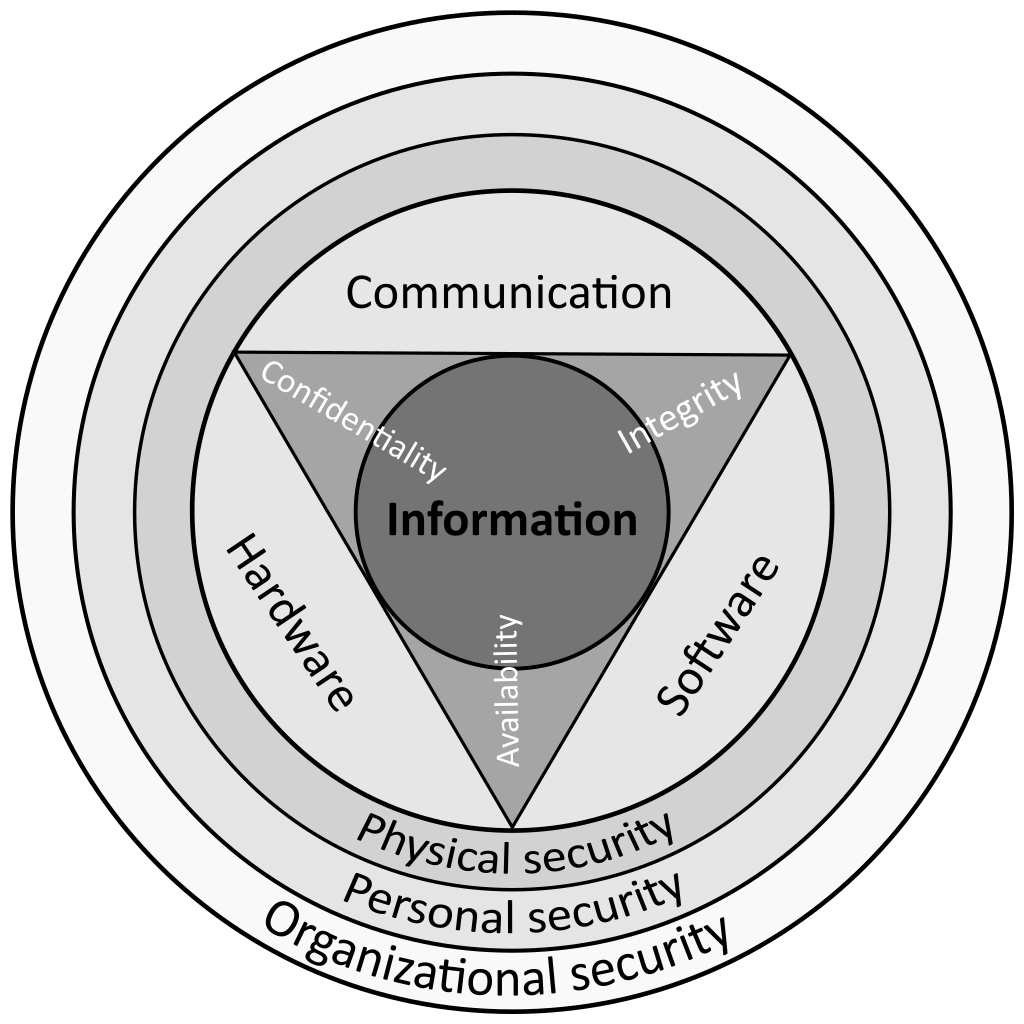
\includegraphics[scale=0.2]{latex/kuvat/ciatriad.png}
    \caption{The CIA-triad, a way to demonstrate conflicting security measures \cite{hughes2013quantitative}. (https://en.wikipedia.org/wiki/Information_security#/media/File:CIAJMK1209-en.svg)}
    \label{ciatriad}
\end{figure}
\subsection{Security by obscurity}

Currently, NixOS is quite rare in both server and desktop usage as shown in figure \ref{timeline}. Combined with the unusual file system and the usage of user-environments, some malware that rely on the usual locations of installed programs may fail \cite{nixosSecurityNixOS}.

\subsection{Multi-user installations}
The requirement for root access nearly always widen the potential attack surface. NixOS provides a way for multiple users installing their programs through the use of user environments, hence mitigating the need for root access. This both lessens the availability aspect, as well as mitigates the programs root access. When file changes are made in user-specific scope, a thin layer of isolation is achieved. \cite{nixosNixOSManual}

\subsection{Data integrity}
Data integrity is achieved both by installed programs residing in the read-only nix store, but also them having been checked against SHA256 checksums. Moreover, the core installation resources for NixOS are GPG-signed by an administrative Nix team. \cite{nixosSecurityNixOS}\chapter{Proposed architecture solution} \label{architecture}

For gaining data points for the research, a test setup must be
configured. This chapter presents a Nix ecosystem, which goes through
a red–blue team testing in chapter \ref{analysis}. The proposed
architecture solution uses a completely declarative approach
introduced in section, where pros and cons of both approaches are
discussed \ref{declarativesystems}.

The proposed architecture is a referential framework for a Nix
ecosystem and provide only a basis for a subset of features needed in
such system. For example, remote access and tunneling would require
extra work in a production setting. Note that presented solution's
scalability could be improved with the use of tools referred in
section \ref{nondeclarative}.

The main purpose of the architecture is to construct a system that
focuses on reliability and fluid deployment tasks. Kandoi and Hartke
discuss the operating large scale IoT solutions through declarative
configuration APIs and conclude that it can solve multitude of
scalability and extensibility challenges of IoT systems thus ensure
reliable and safe operations \cite{kandoi2021operating}. As embedded
security is the focal point of this thesis, a further analysis is
presented in chapter \ref{analysis}.

\section{Server}

Some approaches, i.e by Van der Burg et al. provide a reference
architecture with OpenSSH, Quake 3 server and Transmission services
\cite{van2013reference}. Dolstra, Vermaas and Levy build a declarative
system with simple web server \cite{dolstra2013charon}. This thesis'
server has is moderately complex in comparison with these approaches,
as it contains multiple components and a functioning server–client
implementation.

A proposed architecture can be viewed in figure
\ref{parchitecture}. In simplicity, the NixOS server runs a
MQTT-broker for publishing images encoded in base64 format for the
client devices. The clients are called as device fleet, and the server
is called central server. The client devices submit to configured
topics, and display them using a Wayland compositor, Weston.

The central server has two main functions: receiving SSH-connections
for admin usage and forwarding bitmaps formatted in base64 to the
clients. In production environment, the server would be the element
that is in a public network, and the devices would be accessible
locally (through a tunnel). SSH-connections to the machine would then
be forwarded through the central server to the clients. The central
server currently doesn't generate the imagery, but this could be
achieved via headless browser, or other graphical tools.

MQTT is a extremely lightweight, machine-to-machine publish/subscribe
protocol. It can be used on virtually every platform including
microcontrollers \cite{oasisopenMQTTVersion}. The chosen MQTT broker
and client for this project is Mosquitto. The following snippet shows
how the Mosquitto server is configured in the NixOS server.

\begin{lstlisting}
    services.mosquitto = { enable = true; listeners = [ { users.<user>
          = { acl = [ "readwrite #" ]; }; settings = { cafile =
            "<ssl-path>/ca.crt"; certfile =
            "<ssl-path>/myhostname.crt"; keyfile =
            "<ssl-path>/myhostname.key"; }; } ]; };
\end{lstlisting}

The ''services'' statement tells us that a SystemD service is being
defined. The settings section specify which certificate and key files
are to be loaded to the service.

The MQTT-broker (Mosquitto in this case) publishes a message that is
forwarded to the subscribing clients via a following script.

\begin{lstlisting}
nix shell nixpkgs#mosquitto --command mosquitto_pub -h localhost -t
images/test -m "$IMG_BASE64"
\end{lstlisting}

Sending could be automatized with a service using SystemD timer:
\begin{lstlisting}
    systemd.timers.publish-image = { timerConfig.OnCalendar = "*-*-*
      *:*:00"; wantedBy = [ "timers.target" ]; };
\end{lstlisting}

which invokes a specified service.

\section{Client}

Some IoT solutions prefer client's such relationship with client and
server, where the client automatically searches for suitable server
dynamically \cite{kandoi2021operating}. This thesis' client structure
is static meaning it follows static addresses and forming initial
connections requires manual intervention.

Both server and client are running NixOS. The client has two main
functions: subscribing to media receiving and displaying the gained
media which can be arbitrary. Currently, the image refreshes every
second and through configuration, technically even displaying
animations with this setup could be possible. Media display happens
with feh, an image showing tool, that works with X server. However,
this example is using Wayland, so compability layer XWayland must be
used \cite{waylandWayland}. Image data messaging functions through
MQTT-protocol, which is explained in the next subsection.

\subsection{MQTT-client}
The MQTT client subscribes to a topic from the following script. The
image is received as base64 string, and is converted back to PNG
format.
\begin{lstlisting}
IP="<server ip>" TOPIC="images/test" nix shell nixpkgs#mosquitto
--command mosquitto_sub -h $IP -t $TOPIC >" <image directory path>
/image.base64" base64 -d "<image directory path>/image.base64"
>images/latest.png
\end{lstlisting}
\subsection{Weston/XWayland}
Wayland is a display protocol aiming to replace partially or fully the
old X window system. Wayland functions thorugh a "compositor"
(server), and that provides a surface for the device to draw
graphics. Wayland was selected for this project due to increased
security, as the X window system has support for network transparency
which broadens the attack surface. Wayland has combined server and
client rendering with the Wayland compositor, so that safety-critical
throughput between display server and window manager is not a
concern. \cite{waylandWayland} %% waylandmanual

The example project displays an image from a directory via script:
\begin{figure}[H]
\begin{lstlisting} 
    sleep 5 && /nix/store/qc9j6pm6ykyx531s4kb06084mczy2l6g-feh-3.10.1
    /bin/feh -F -Z -R 1 <image-path>/latest.png
\end{lstlisting}
\label{fehscript}
\end{figure}
As the programs must be found from an absolute path, the system must
generate the scripts accordingly. This is done via a SystemD service,
specified as:



\begin{figure}[H]
\begin{lstlisting} 
    { config, pkgs, ... }: let fehLaunch = pkgs.writeText "feh.sh" ''
    echo "sleep 5 && ${pkgs.feh}/bin/feh -F -Z -R 1 <image
    directory>/latest.png" > /home/user/abzug-receiver/weston/img.sh
    ''; initImg = pkgs.writeText "initImg.sh" '' echo
    "${pkgs.gcc}/bin/gcc <source path> img.c -o <binary path>/img" >
    /home/user/abzug-receiver/weston/init.sh '' in {
      systemd.services."westonl" = { enable = true; unitConfig = {
          Type = "oneshot"; }; serviceConfig = { Environment =
          "XDG_RUNTIME_DIR=/var/run/user/1000"; ExecStartPre =
          ["${pkgs.bash}/bin/bash ${initImg}" "${pkgs.bash}/bin/bash
            <init.sh path>/init.sh" "${pkgs.bash}/bin/bash
            ${fehLaunch}" "${pkgs.bash}/bin/bash <init.sh
            path>/init.sh"]; ExecStart = "${pkgs.weston}/bin/weston
          --config=<weston configuration directory>/weston.ini";
          RestartOn = "failure"; }; wantedBy = [
          "graphical-session.target" ]; }; }
\end{lstlisting}
\label{systemd1}
\end{figure}

This wouldn't be a problem in traditional Linux distribution, but in
NixOS the program locations vary from machine to machine
\cite{dolstra2010nixos}. A program resides in Nix store, with a
cryptographic hash of all build inputs in its directory
path. \cite{dolstra2010nixos}. For that reason, one way of proceeding
is to write a SystemD service to generate the configuration
files. Note that this SystemD configuration differs in how SystemD
scripts are declared usually. Most SystemD distributions have SystemD
files in /lib/systemd/system directly or via symbolic link.

In the beginning of the configuration, variables are defined and
program locations are expanded from Nix package paths. Then, in the
''serviceconfig'' part of the configuration, the strings are forwarded
to shell, which in part compiles sources and executes scripts. After
the ''ExecStartPre'' section, in the ''ExecStart'', Weston is launched
with very basic kiosk configuration:

\begin{figure}
\begin{lstlisting} 
  [core]
  idle-time=0 xwayland=true
  [shell]
  panel-location=""
  panel-position=none**
  [autolaunch]
  path=<feh launcher path>/img
\end{lstlisting}
\label{westonconf}
\end{figure}

the ''[autolaunch]'' only functions with compiled binaries thus the
shell script is not directly executed. Instead, a program written in C
is invoked, which in part invokes the shell script with
parameters. The autolaunch path can handle switches, but unfortunately
not parameters. With these workarounds the kiosk successfully can
display media as shown in figure \ref{testimage}. Feh is launched with
-R 1 parameter, which causes it to refresh the image every
second. That way when a new image is uploaded, the display is also
refreshed.

\begin{figure}
    \centering 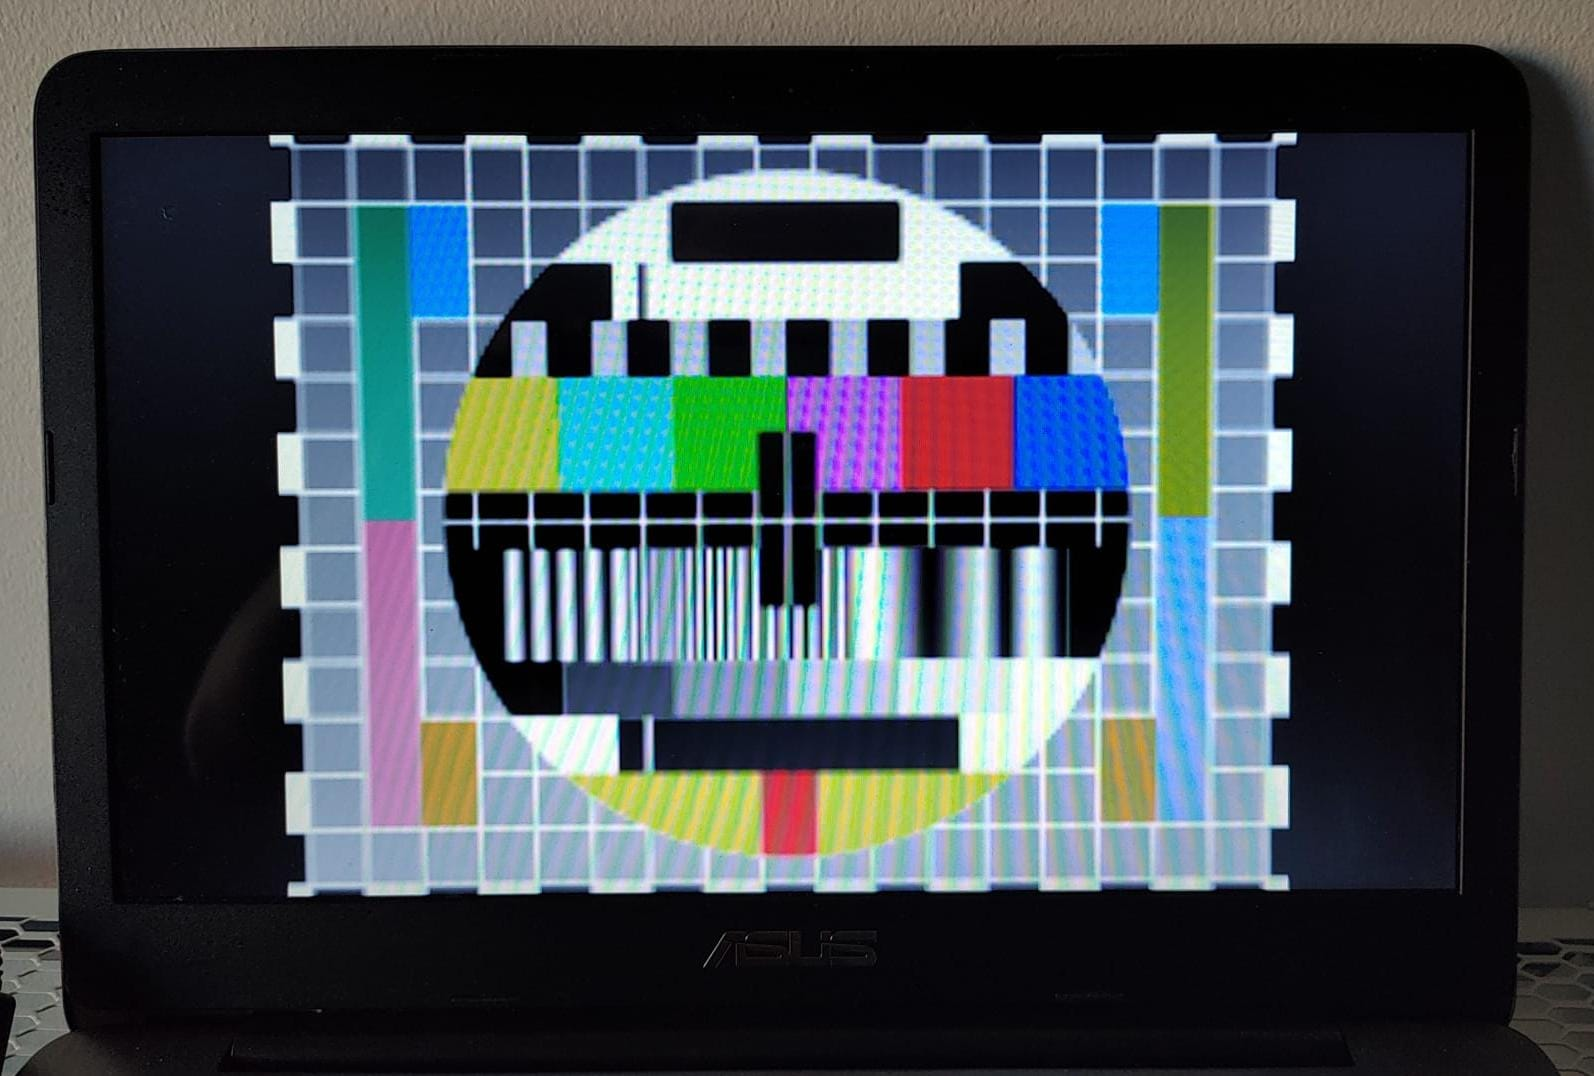
\includegraphics[scale=0.2]{latex/kuvat/testimage.jpeg}
    \caption{Working example of a NixOS client displaying image with
      Wayland and Feh.}
    \label{testimage}
\end{figure}

The sources and scripts are downloaded from Github, again via a
SystemD service. Following snippet shows the "ExecStart" part of the
service.

\begin{lstlisting}
ExecStart="${pkgs.git}/bin/git clone <git url> <installation path>";
\end{lstlisting}

%\begin{figure}[t!]
%\centerline{\includesvg[width=0.70\columnwidth]{latex/kuvat/thesismain.drawio.svg}}
%\caption{Architectural graph of the test setup.}
%\label{parchitecture}
%\end{figure}

\begin{figure}
\includesvg{latex/kuvat/architect.svg}
\caption{Architectural graph of the test setup.}
\label{parchitecture}
\end{figure}
%\begin{figure}
%    \centering
%    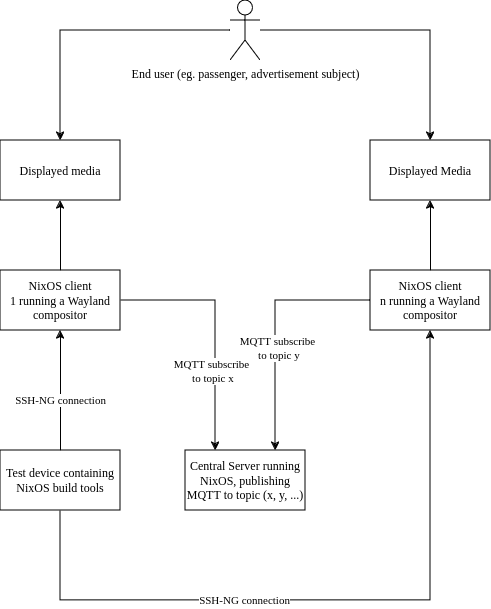
\includegraphics[scale=0.8]{latex/kuvat/architecture.drawio.png}
%    \caption{Architectural graph of the test setup.}
%    \label{parchitecture}
%\end{figure}

This part of the configuration is not purely functional, as the
downloaded scripts and configuration can be arbitrarily changed with
correct permissions. The SystemD services impurity don't trigger the
Nix language evaluation itself, so ''--impure'' switch isn't
mandatory.

\section{Test device}

A huge benefit from declarative systems is their broad possibilities
of automated system tests \cite{van2010automating}. The phrase: "if it
works on one machine, it will work on another" builds a stable
foundation for such tests \cite{nixosNixOSManual}. Different
deployment strategies benefit from slightly different approaches, but
as deployment strategies generally are out of this thesis' scope, only
a minimal test setup is configured.

NixOS devices can be upgraded and updated through a server or locally
with physical access \cite{nixosNixOSManual}. In this thesis' example,
a separate test machine is configured, and it's programs are
replicated to other devices as seen on figure
\ref{parchitecture}. Updates are done manually with command:

\begin{lstlisting}
nix build --eval-store auto --store ssh-ng://remote-host
\end{lstlisting}

The test device is thus replicated to all remote hosts manually, but
an automation script would be useful as the setup scales.

\section{Installing new devices} \label{instnewdevices}

Installing devices could made trivial, as it's trivial to generate new
NixOS images from pre-existing configuration files
\cite{nixosNixOSManual}. The problem is, however, that in many cases a
legacy architexture exists, which needs to be overwritten. This
section focuses on research question 3, providing a solution for
migrating from existing architectures.

If the whole setup needs to be replicated to an existing device fleet,
a great help would be open source project ''NixOS anywhere''. NixOS
anywhere specifies minimal specifications: ''Unless you're using the
option to boot from a NixOS installer image, or providing your own
kexec image, it must be running x86\_64 Linux with kexec
support. Fortunately, most modern x86\_64 Linux systems have kexec
support. By providing your own image you can also perform kexec for
other architectures e.g aarch64''. NixOS anywhere also has a
requirement that the devices should be available at a public network
(not only wireless LAN), which wouldn't probably be a problem in
production environments. NixOS anywhere also works only with NixOS
flakes, so this thesis' configuration would need to be contained in a
flake. \cite{githubGitHubNixcommunitynixosanywhere}
%% cite nixos manual
The installation would contain the following steps:
\begin{enumerate}
  \item Run ''curl -L
    https://github.com/nix-community/nixos-images/releases/download/nixos-unstable/nixos-kexec-installer-noninteractive-x86\_64-linux.tar.gz
    | tar -xzf- -C /root /root/kexec/run'' for booting separate kernel
    for installation.
  \item Generate a minimal configuration file: ''nixos-generate-config
    --no-filesystems --root /mnt''
  \item Add ssh-keys to the configuration
  \item Upload the flake from the server to the device ''nix run
    github:nix-community/nixos-anywhere -- --flake <path to
    configuration>#<configuration name> root@<ip address>''
\end{enumerate}
Another way would be setting up NixOS from the installation media and
setting up manually or creating a installation media with Nixos
generators project
(https://github.com/nix-community/nixos-generators). Nixos generators
is available from Nixpkgs, and can thus be installed to a NixOS
development machine or server. Invoking
\begin{lstlisting}
nixos-generate -f iso -c <configuration.nix path>
\end{lstlisting}
would result in a ISO format image, ready for
installation. \cite{githubGitHubNixcommunitynixosanywhere}
 \chapter{Security standpoints} \label{securitystandpoints}

Security is inherently challenging to measure adequately due to its
complex and chaotic nature. Qualitative analysis may also result in
subjective output. As such, no unambiguous standard of measuring
security can be provided \cite{wang2005information}. To overcome these
challenges, several metric systems are compared and the one that
provides the most precise answers specifically for this thesis' cause
is chosen.

In this chapter, a selection process for meters which in part are used
for gaining quantified data, is presented.  When finally quantitative
metrics are gained with the help of two paradigms, GQM (goal, question, metric) and
specifically its superset SMART, a red–blue team layout is erected
using QuERIES methodology. SMART is used in conjunction with the
literature review to reveal the most suitable methodology for this
thesis. SMART is opened more in the section \ref{choosingsecmet}.

Using an exact metric system is important, as this this thesis'
emphasis is on measuring the security of a declarative approach. The
presented architecture in the previous chapter works as an example on
how a declarative system can be improved by reconfiguration, utilizing
a red-blue team setup.

\section{A brief history of security metrics}

The history of security metrics begin from Trusted Computer System
Evaluation Criteria (TCSEC) also known as the Orange Book from 1983,
which popularized many terms still in use today such as
identification, authentication and
authorization. \cite{bayuk2013measuring}

In the 1990s, when the US National Bureau of Standards (NBS), later
known as the National Institute of Standards and Technology (NIST),
tried to standardize security, it became clear that systems needed to
adhere closely to the definitions outlined in the Orange Book and the
subsequent Common Criteria project. Over time, various other standards
gained popularity, such as the System Security Engineering Capability
Maturity Model (SSE-CMM), which serves as a checklist for system
design from the ground up. \cite{bayuk2013measuring}

Later it was observed, that systems design is only a part of a
successful security strategy and operational practices played a
bigger role than expected. This was something to be addressed in 1995 NIST
Computer Security Handbook which evolved to provide ground to
combat modern issues. \cite{bayuk2013measuring}

As metrics can be used as a tool for decision making, the strategical
approach of the mentioned publishes is important. It is noteworthy, that
the strategies (the Orange Book, SSE-CMM, etc.) begin to measure
security by compliance to defined ratings. Later in 2000s more
mathematical approaches were taken, one which is delved deeper in
section \ref{whyqueries}. \cite{bayuk2013measuring}

\section{Choosing security metrics} \label{choosingsecmet}

Security is something that is challenging to measure due to its
complex nature. A GQM (Goal, question, metric) paradigm helps to
choose appropriate metrics: first there must be a set goal to an
organisation, then a formulated question for each goal. These answers
are then reflected to gain the desired metric. This strategical
approach is perhaps too broad for this thesis' scope, but it aligns well
with a usual organisational strategy. \cite{papazov2019cybersecurity}

A more appropriate tool for this task would be SMART – a set of inputs
to evaluate meter systems' suitability. These inputs describe how
specific, measurable, attainable, relevant and timely the methodology
is \cite{payne2006guide}.

In cyber security, being specific is very important. A common issue
with security meters is, that they either cover too many topics and
are without precise definitions or they are too specific to be
generalized to a broader scope of situations
\cite{wang2005information}. The results of this thesis are crucial to
measure, as the research focuses on system states and aims to assess
the outputs produced by state transitions.

The concept of attainability is important in this context because this
thesis has a narrower scope compared to a large
organization. Therefore, the proposed setup must be evaluated to
ensure that the metrics' goals are achievable. Relevance has to do
with risk assessment and how important it is to measure something related
to it's value. Risk assessment is explored in detail  in chapter
\ref{analysis} section \ref{modprob}. Time-bounding signifies the
importance of time as a meter; a system that can be penetrated in a
minute can certainly be seen as weaker than a system that takes years
to be compromised.

\section{Measuring security} \label{measuringsecurity}

In this section, different methodologies and perspectives gained
through literature review for cybersecurity are discussed, and
potential methodologies are compared to gain the most adequate metric
system for usage through SMART process \cite{payne2006guide}.

Security metrics can be categorized into four themes:
\textbf{system vulnerabilities}; measuring vulnerabilities can be
applied to user-related, interface-induced, password, and software
vulnerabilities. Users are constantly at risk of threats such as
phishing attacks or malware infections, where the user of any system
becomes the primary attack vector. Interface-induced vulnerabilities refer to attack vectors associated with open ports
and endpoints. \cite{pendleton2016survey}

Password vulnerabilities refer to instances where a password can be
cracked through computational methods. This is fairly easy to measure,
as it is possible to estimate the time required to crack a password or
assess its vulnerability using statistical password
guessability. Software vulnerabilities are a common cause of security
breaches. These vulnerabilities can be measured and estimated based on
past exploitations. A key metric in this context is the time taken to
patch a software vulnerability. \cite{pendleton2016survey}

\textbf{Defense} measures can be applied to strengthen reactive,
preventive, proactive and overall defenses. Reactive measures include
blacklisting which is a lightweight mechanism to prevent e.g for preventing botnet to harm
the protected system by blacklisting IP-addresses related to the
botnet. For measuring defence, the reaction time is essential and
most importantly, it is a gained meter to measure preventive
defense. Blacklisting can also be used as a preventive and a proactive
measure, as a pre-filled blacklist can be used with desired
parameters. \cite{pendleton2016survey, ramos2017model}

Overall defenses can be measured with the combination of all defensive
measures and with the use of penetration testing in a red–blue team
setup. Penetration testing aims to gain a result, also known as
penetration resistance, which is a meter indicating cost or time that
the red team must spend in case of a successful system
compromisal. \cite{pendleton2016survey, ramos2017model}

\textbf{Threats}: zero-day vulnerabilities can be measured from two
perspectives: lifetime of zero-day vulnerability and the number of
nodes that are compromised as a result. Malware spreading can be
traced with the parameter infection rate, which is defined as infected
node per a time unit. Attack evasion is assessed using either the
obfuscation prevalence metric or the structural complexity
metric. These metrics offer insights into the obfuscation of acquired
samples, such as through encryption, or the complexity of the target
system, which is measured by its runtime. \cite{pendleton2016survey,  ramos2017model}

\textbf{Situations} can refer to the security state, security
incidents, and security investments. The security state encompasses
various parameters, such as the incident rate and the blocking
rate. Security investments,  measure the percentage
of the budget allocated to security and the return on those
investments. \cite{pendleton2016survey}

\section{Methodologies in comparison} \label{whyqueries}

Cybersecurity metrics based on quantified
mathematical models, which are prevalent for this thesis exist today. Three
different methodologies are discussed, and one is picked for measuring
the security of this thesis' architecture implementation. All the following metric
systems are \textbf{measurable}. However, some fit better in relation with \textbf{time-related} and \textbf{relevance} axes.

The literature review provided three central methodologies from different perspectives. Complex mathematical models
presented by Alshammari et al. are too broad
\cite{alshammari2009security}. This thesis' scope is limited and this
methodology would fit better in a wider cyber security setting.

A methodology based on object-oriented thinking and UML diagrams is
suitable in many contexts. However, as mentioned in the paper, this
measurement methodology is used to compare similar alternative designs
\cite{alshammari2009security}. As noted, the focus of this thesis is
not comparative, since all critical comparisons have already been made
in chapter \ref{imperative}.

The Hidden Markov models presented by Wang et al. are closely aligned
with the end goal of this thesis \cite{wang2010framework}. The
time-related aspect is suitable, as the Hidden Markov model
incorporates a time parameter. However, the issue lies in the
generality of the methodology, and a more specific approach would be
better suited for this thesis. Nevertheless, we apply a similar
approach to that of Wang et al. for calculating the POMDP parameters.

The last and the most fitting methodology would be the one presented
in papers by Carin et al. and Hughes et al.
\cite{carin2008cybersecurity, hughes2013quantitative}. The QuERIES
methodology is delved deeper in section \ref{querieschapter} and its
time-related, relevance and specific axes are a near-perfect match for
our goals as the model itself is relatively simple and provides
shifting probabilities from states, which serves this thesis' study
design well.

\section{Quantitative metrics} \label{quantitativemetrics}

Carefully selecting a metrics system includes asserting our goals and
questions. Our goal is to discover this thesis' architecture proposals'
tenacity in a simulated setting. The main goals reside in this thesis'
two research questions:

\begin{itemize}
\item How can a declarative system be used to measurably improve the basic
  security needs of an embedded system used for displaying public
  media?
\item What are the advantages and/or disadvantages of such system from
  system administrator standpoint?
\end{itemize}

The proposed architecture solution presented in chapter
\ref{architecture} will go through a red and blue team inspection,
complying with the QuERIES model in chapter \ref{analysis}.

\subsection{QuERIES} \label{querieschapter}
QuERIES model consists of number of steps that

\begin{enumerate}
  \item model the problem - by conducting a risk assessment of the
    attack surface and the value of the possible intrusion
  \item model the possible attacks - build an attack graph of
    intruding though vulnerabilities or other means
  \item quantify the models - by conducting a controlled red team
    attack and provide quantified results for the said attack
  \item use the results - use blue team methodologies to provide
    increased protection against the exposed problems
  
\end{enumerate}

First, the blue teams' task contains the risk assessment of the attack
surface. It is particularly important for the blue team to acknowledge
the most crucial points of the attack surface, that is also used as
the base for quantitative analysis. As seen in figure
\ref{queries}, the methodology is applied \textit{iteratively}, i.e
the steps are repeated as many times as needed for the system to be
secure.

Modeling the possible attacks is a task for the red team – by
constructing an attack graph, the opposing forces have a plan which
can be used as a template for analysis. In this thesis, the models are quantified with the use of time
framing. Both teams have a limited amount of time to conduct their
tasks and the probability for succeeding a certain task is calculated
with the following formula

\[ \frac{t_e}{t_t} \]

where \(t_e\) stands for elapsed time and \(t_t\) for maximum time
that can be used which is the same for all tasks.

\begin{figure}[t!]
\centerline{\includesvg[width=0.50\columnwidth]{latex/kuvat/queries.drawio.svg}}
\caption{The QuERIES methodology is used as a reference flowchart for
  evaluation of security. \cite{hughes2013quantitative}}
\label{queries}
\end{figure}
\subsection{QuERIES as a central methodology} \label{queriesasmethodology}

QuERIES draws inspiration from computer science, game theory, control
theory and economics, thus is a complex answer to a complex
question. It is stated, that it can be used as an alternative to
popular methodologies such as red teaming or black-hat analysis, used
commonly in risk-assessment. \cite{carin2008cybersecurity}

QuERIES is proposed to have potentially significant usage in DoD
(Department of Defense) and in the private sector
\cite{carin2008cybersecurity}. Initial testing of QuERIES in
small-scale and realistic scenarios presented by Carin et al. suggest
that the methodology can in fact be used as to improve risk-assessment of
more complex settings \cite{carin2008cybersecurity}. This thesis
follows similar steps: first the QuERIES methodology is used to assess
risks followed by generalization with strict constraints in mind.

As stated by Hughes et al. the result of QuERIES isn't binary: the
attacker must think about the most optimal timeframe to stop the
operation \cite{hughes2013quantitative}. The strategy uses
\textbf{open} and \textbf{closed} loop decision algorithms for
deciding when to stop trying. Closed loop decision algorithm
constantly evaluates when is the optimal time to stop trying and open
loop means that the system has pre-defined goals for evaluation
\cite{carin2008cybersecurity}. As a positive side-effect, by gaining
the probabilities through red-team evaluation, the system is
thoroughly tested and improved. This is a valuable metric, offering
insight into how the value of the system changes over time in terms of
the cost of breaching it, thereby reflecting the true cost of the
attack. As stated by Hughes and Cybenko, if the value is high enough
related to the value of the gained value, they will
perform the attacks less likely \cite{hughes2013quantitative}.

In this thesis, the value of the whole system architecture is
defined as 1, constituting a value of holded intellectual
property (IP). Costs are defined as fractions of the value, deflating 
0.1 every hour. This is contrary to the original paper where the
value of the intellectual property has a certain value of 30 000\$, and
the value for the possible intruder is defined as 60\$ per hour
\cite{carin2008cybersecurity}. This divergency is due to the fact
that it is impossible to define a certain value for our system.
It also provides clarity as it is ergonomic to see how an attack
estimates the relation to the value of the intellectual property. 

\subsection{Partially observable Markov decision process}

Lastly, using the results of the POMDP can be used to increase the
protection against the discovered problems
\cite{carin2008cybersecurity}. The original QuERIES methodology used
economic models for estimating POMDP parameters instead of
calculating them manually \cite{carin2008cybersecurity}. We gain the
parameters from POMDP by calculating state transitions with given
observations. Attacks and defenses are quantified through a partially
observable Markov decision process (POMDP) which contains the following six
steps:

\begin{enumerate}
    \item Define possible states the system can be in
    \item Define the actions the system can take
    \item Define the possible observations the system can take
    \item Define the transition probabilities of the system
    \item Define the observation probabilities of the system
    \item Rewards: guide the system towards the desirable actions and
      states.
\end{enumerate} \cite{hughes2013quantitative}

A POMDP is used widely in these kinds of applications, as both blue and
red teams have only partial observations in relation to the system
\cite{mcabeeMarkov}. The blue team can't be completely certain that
the system is secure, and the red team cannot perform fully reliably as
systems and environments differ from each other. As mentioned in the
previous section, the focus of the QuERIES analysis is the time to
reverse-engineer the system thus emphasizing the importance of only
partial observations.

In the next section the architecture presented in chapter
\ref{architecture} is improved using the applied QuERIES methodology. An
attack graph is constructed and POMDPs are utilized. The result will
provide information about the architecture's security, and it will
undergo several iterations of the QuERIES pipeline with each improving
the overall security of the system.
 \chapter{Applying QuERIES} \label{analysis}

As mentioned in the previous chapter section \ref{queries}, the
QuERIES inspired methodology is used in this chapters analysis. In
table \ref{pomdbtable} is listed all the possible states (S), defender
actions (D), attacker actions (A) and observations (O). Then, every
transition from state to another state is calculated as a probability.

QuERIES as a model is described as multidisciplinary, as it takes
inspiration from traditional red-blue team approaches, mathematical
models to economic models \cite{hughes2013quantitative}. In other
literature, particularly by Bojanc and Jerman-Blažič, it's argued that
modeling cybersecurity with economic models can provide substance for
minimizing risks organization-wide \cite{jerman2008economic}. In this
chapter, we will apply the model and discuss the implications in both
security and economic standpoints. The main focus however is on how
using QuERIES, we can improve the security of the architecture.


\section{Modeling the problem and quantifying the models} \label{modprob}

The example project of this thesis is an image showing architecture that
could be used e.g for advertisement, public transport timetables or
practically anywhere where static media should be presented. Our use
case focuses on displaying arbitrary media in a public location. The
results, if an an intruder should gain unauthorised access, would be
anywhere from displaying explicit imagery to succeeding in displaying
propaganda or other unwanted content. Unauthorised access would have a
negative economic effect for the service provider, as every
organisation displaying media want to remain credible among
stakeholders.

The attack surface of the example project focuses on physical access
and vulnerabilities in remote connections. With MQTT-messaging, SSH
and display protocols, internal and external messaging takes place.

As mentioned in chapter \ref{securitystandpoints} section
\ref{measuringsecurity} subsection \ref{queriesasmethodology}, the
value of intellectual property is defined as $\alpha$, for which other
parameters refer to as fractions of it. If this was applied to a real
setting, the value of intellectual property would be calculated
appropriately for the scenario.

\section{Modeling the possible attacks}

In this section, the possible attacks are modeled using an attack
chart, depicted as a POMDP, which is a modeling tool presented
earlier. In the original paper where QuERIES is presented, an
important parameter is the time to reverse-engineer the system without
prior information about the protection scheme
\cite{carin2008cybersecurity}. Our approach is different; the attacks
are considered as successful, if they gain further leverage in the
attack graph, e.g transitioning state ''idle'' to ''partial loss of
system''. This is to maintain cohesion in the study, as we don't need
to define what it means to ''reverse engineer'' the system. In this
case, information of the system is publicly available as an open
source project, thus the information of the system being available
also to the attacker.

In table \ref{pomdbtable}, the first column describes states the
system can be in. The second and the third column state defensive
actions, and observations of the system. The fourth column contains
template of the attacks that could be conducted. After forming the
attack graph depicted in the table, the attacker tries to breach the
system, leveraging through the A0-A4 column. The probabilities are
then calculated with the model presented in chapter
\ref{securitystandpoints} section \ref{quantitativemetrics} subsection
\ref{queries}.

The algorithm produces a reward value for each QuERIES iteration,
which is used to improve the setup. For calculating reward values, R
script with library ''pomdp'' was used.

\begin{landscape}
\begin{table}
\centering
\begin{tabular}{ |c|c|c|c| }
 \hline & & & & S0-S7 & D0-D4 & O0-O4 & A0-A4 \\ & & & & \hline \hline
 & & & & Idle & Monitor system & Normal operation & Intercept MQTT
 messaging \\ & & & & \hline & & & & Receive media through MQTT &
 Isolate system & Detected suspicious activity & Compromise Github
 repository \\ & & & & \hline & & & & Set up SystemD services &
 Shutdown system & Detected unauthorised access & Gain physical access
 to device \\ & & & & \hline & & & & Start Weston & Isolate device &
 Detected unusual media display & Exploit vulnerabilities in display
 \\ & & & & \hline & & & & Display media & & & Exploit vulnerabilities
 in SSH connections \\ & & & & \hline & & & & Partial loss of system &
 \ & \ & \\ & & & & \hline & & & & Complete loss of system & & & \\ &
 & & & \hline & & & & & & & \\ & & & & \hline

\end{tabular}
\caption{Different states, defensive measures, observations and attack
  measures for the system.}
\label{pomdbtable}
\end{table}
\end{landscape}

A weight of 1 was used for positive results, and -100, if something
was to be compromised. This weight distribution is due to the fact
that even if blue team succeeds most of time, the results of failure
are much worse than a succeeding result from the blue team. The
discount constant is used in calculations as shown in appendix 
\ref{pomdpappenix}, where it influences the priority of immediate
versus future rewards \cite{mcabeeMarkov}. Our case signifies the
importance of both, so value of 0.75 was used. Note that the maximum
reward value is 4, and the minimum is -400.

\section{Using the results} \label{usingtheresults}

The results are investigated through the probabilities, which are
represented in the table. The reward score is taken in account on how
successful/unsuccessful the setup is from a security perspective. The
score itself is rather abstract; it's main function is to demonstrate
the \textbf{overall security} of the architecture. In short, negative
numbers imply there are flaws in security, and positive numbers mean
that the system is more secure
\cite{mcabeeMarkov}.

As stated by Hughes and Cybenko, using the results means evaluating
the gained results to decide if proposed protections are adequate for
our means \cite{hughes2013quantitative}. The QuERIES model was
iterated 2 times, and the results were placed in the following table.

\begin{table}[h!]
\centering
\begin{tabular}{|c|c|c|}
  \hline Iteration & Reward function & Proposed protections \\ \hline
  1 & -25 & Multiple \\ \hline 2 & 4 & None \\ \hline
\end{tabular}
\caption{Protections applied in each iteration}
\label{iterationtable}
\end{table}

The reward function in the first iteration is calculated with the
script. The second value is calculated
with as the maximum accumulated points; the highest value is 4 points
without any discount, as the red team failed to provide any results
for the second iteration. This is partially due to time limit, as in
the test set up there was only one attacker with very limited time. I
argue that with more time, it would have been possible for the
attacker to breach.

As seen, the reward function is growing as the proposed protections
are applied in each iteration. In the following figure
\ref{timetobreach} we can see that the time to breach peaks in the
first hour.

\begin{figure}[t!]
\centerline{\includesvg[width=1.0\columnwidth]{../graph/barchart.svg}}
\caption{Probabilities to breach into the system.}
\label{timetobreach}
\end{figure}

The time distribution of breaches are depicted in the graph
\ref{timetobreach}. The chart has similar shape as the chart in
\cite{carin2008cybersecurity}, meaning that attacks in their initial
phase succeed more frequently at least in these two cases. The following chart is used to decide, when is the
optimal time to stop the attacks from the attacker perspective. We use
this also to reflect the cost estimate of the blue team. Following the
methodology in referred papers by Hughes and Cybenko, the optimal time
to stop the attacks is seen in the following graph using open and
closed loop strategies \cite{hughes2013quantitative,
  carin2008cybersecurity}.

This economic model can be used to generalize risk in this kind of
situations. In the following graph \ref{openandclosed} we can see that
the cost for the attacker peak at about 6 hours using closed algorithm, and
at 3 hours using open algorithm. Open loop algorithm means that the cost
estimate never evaluates feedback from a system
\cite{bars2006theory}. Closed loop behaves in an opposite manner; it
constantly modifies its behaviour based on the feedback it gets \cite{bars2006theory}.

We can see that with closed loop algorithm, the attacker can gain more
results with worse cost tradeoff, but with open loop, it gets
immediate results with cheap cost. This could be important for the
holder of the intellectual property, as it must protect itself against
attackers using both algorithms. In our case, where the potential
threats are e.g hacktivist groups, the cost estimate doesn't matter as
much. Therefore, it's important to be aware that an attacker which
doesn't have economic interests, could have practically unlimited time
to try to breach the system.

\begin{figure}[t!]
\centerline{\includesvg[width=1.0\columnwidth]{../graph/cost_graph.svg}}
\caption{Cost benefits and reductions. The black dots indicate the
  most optimal times to stop the attack.}
\label{openandclosed}
\end{figure}

\subsection{Improving the system using Nix}

The following measures were taken in the first iteration: disable USB
ports, change MQTT password to token based authentication and change
SSH to key based authentication. As we can see, the QuERIES output
provided concrete results on what are the weak points of the system.

As an example, the exposed USB-ports of the system were found to be a
problem, due to the possibility of infecting the system with direct
control to the system. This can be mitigated easily by modifying the
client devices configuration.nix, with the following changes:

\begin{figure}[H]
\begin{lstlisting} 
{ boot.kernelPackages = pkgs.linuxPackages_latest; boot.kernelParams =
  [ "nousb" # Disables USB at the kernel level ]; boot.kernelModules =
  [ ]; boot.extraModulePackages = [ ]; services.udev.extraRules = ''
  SUBSYSTEM=="usb", ACTION=="add", OPTIONS+="ignore_device" ''; }
\end{lstlisting}
\label{kernelsnippet}
\end{figure}

The configuration could be applied to any number of clients, proving
that Nix could be used to rapidly address arising security
issues. This supports the argument presented in chapter
\ref{imperative}, that through updatability the security could be
improved. The configuration is only an example to mitigate hardware
access attack vectors, as there are many more ways for the attacker to
leverage the access, e.g by replacing the whole device, depending on
the resources of the attacker. This highlight the scalability of Nix
systems; it doesn't matter if we have one or thousands of devices,
updating them is equally simple. A huge contrast between imperative
and declarative systems is found, as imperative systems would need
linear administration time in relation with the number of devices.

\subsection{Issues with QuERIES} \label{issues}

One issue found using QuERIES with POMDP was that applying the reward
functions is in our case rather arbitrary. We assumed, that for
positive results, the reward function is defined as 1, and for the
negative outcomes -100. This is due to the negative results deemed as
catastrophic and the positive results being slightly positive. The
choice for both parameters could have been any integer, but the issue
is that it demands ''gut-feeling'' of the author to select the
appropriate parameters. This could be mitigated with some study on
selecting the paramers, but it's definitely a challenge to provide
good foundation on such abstract numbers.

One remark using POMDP is that it produces very generalized
output. This is why we use methodologies such as QuERIES to improve
the system, POMDP being just one component. Other benefit from using
POMDP is that it provides us concise attack graph, and I argue that
using the POMDP calculations may even be redundant. In POMDP, negative
rewards signify that the system has issues, and positive meaning that
the system is more secure \cite{mcabeeMarkov}. More ergonomic approach
would be calculating rewards without positive outcomes, due to them
possibly shadowing the most critical issues. Developing a pessimistic
model that highlights explicitly the weak points of a system would be
a topic for further research.

\section{Generalizing the results}

The results of this chapter could be generalized to a more complex
setting, using a similar methodology. The POMDP model scales well, if
more parameters would be supplied. This study proves that while
measuring cybersecurity is difficult, remaining in tight constraints
we can get adequate estimates for applying economic models for the red
team, further projecting the risk vs. reward.

Carin et. al \cite{carin2008cybersecurity} argue that QuERIES can be
applied in both public and private sectors to help to improve the
security of both software and hardware. I argue that a hand-tailored
application of QuERIES can be used as a powerful model that is
ergonomic to use in the right hands. However, the use of complex
applied mathematic models require proficency in both cybersecurity and
mathematics, which can be hard to achieve in a real organizational
setting. This is why I propose in the next chapter that a simpler,
pessimistic and more concise model would be easier to reach for an
organization.
 \chapter{Further research} \label{further}

One big limitation of Nix is the fact that it mainly supports only
x86\_64, i686 and arm64 platforms \cite{nixosNixOSManual}. This is not
generally enough, as many different architectures are used in
embedded, thus limiting the use-cases of
NixOS. \cite{fysarakis2014embedded}.

A declarative approach could be used with other processor
architectures. This would require work on a declarative package
manager, which would be used in conjunction with base systems created
with Buildroot or Yocto.

As far as security is concerned, the main methodology of this thesis'
research, QuERIES, proved to be an aqequate tool. It helped to improve
the security of the reference architecture. However, some issues were
raised in chapter \ref{analysis} section \ref{usingtheresults}
subsection \ref{issues}. These issues could be addressed in developing
a new methodology, inspired by QuERIES, providing explicit insight on
the weak points of the underlying system. This approach would be
similar to this thesis' QuERIES inspired methodology.

\section{Further research questions}


Questions for further research include:
\begin{enumerate}
  \item{What kind of new methodology would be more better, reflecting
    the found issues in QuERIES for similar use-case as in this
    thesis?}
  \item What set of tools would be optimal in creating a true
    cross-platform declarative package manager (e.g programming
    languages, possible configuration languages etc.)
      
    \item How could the new system handle common system security and
      administration problems better?
      
\end{enumerate}

These questions form ground for multiple separate studies.
 \chapter{Conclusion} \label{conclusion}

Nix can be a useful base for issuing a purely functional, declarable
systems while providing an advanced rollback mechanism. Configuring it
depending on the system administrator may be gruesome, but it can
dodge the usual pitfalls of more popular systems. While the usage of
Nix language demands proficiency, it is a solution to distribute,
update and administrate more secure systems. NixOS handles
exceptionally easily features such as Wayland and audio driver
setup. In the end, NixOS is very predictable and the statement "if it
works on one machine, it works on another" proves to be true.

Problems presented in this thesis could be solved with many different solutions,
but the Nix approach is rather unique as it makes reproducible systems
very straight forward. As the system is defined in the
configuration.nix file, there's little that could go wrong even when
underlying hardware varies. The same doesn't apply to the mentioned
Debian distribution.

Measuring and improving the architectures solution proved to be
challenging but fruitful. With multiple iterations used with QuERIES,
the architecture developed from insecure to more secure. This is a
testament for applying successfully a certain methodology for a
specific task.

% security implications closing
As far as security implications are concerned, Nix is a good tool for
asserting compliance. In purely functional environment, anything that
needs compliance can be checked from the configuration files. As disk
encryption is trivial and read-only Nix store provides increased
integrity, a more secure system can be achieved also through the
actions of a system administrator. A system administrator must adhere
at to Nix philosophy with the Nix language and as all the configured
parts can be viewed quickly. For example, a question ''what ports are
in use in each client device'' can be answered very quickly and in
precise manner by just viewing the configuration files.

As mentioned, popular embedded Linux distribution creating tools,
Buildroot and especially Yocto have also steep learning curves. They
also lack the ease of updatability provided by Nix, which is a
significant problem regarding security.

The research proved that the purely functional Nix system is easily
updatable and upgradable solution for maintaining a secure system.
While NixOS is a niche Linux distribution, and probably remains as
such, the concepts, however I assume will live on in future. A purely
functional declarative system with atomic rollbacks is something I'll
await to be iterated in the future with further user availability in
mind.


%\input{file_name_of_chapter_x}
%\input{file_name_of_chapter_y}

% The thesis main content ends here.

\printbibliography

\begin{comment}
Important! Create the appendix chapters with command \textbackslash appchapter\{some
name\} instead of \textbackslash chapter\{some name\} for the automagic
page counting to work!
\end{comment}


\appchapter{Partially observable Markov decision process with R} \label{pomdpappenix}

The following R code calculates the result score from the study in \ref{analysis}.

\begin{verbatim}
library("pomdp")

CYBSEC_POMDP <- POMDP(
    states = c("Idle", "Receiving media through MQTT", "Setting up SystemD services", "Starting Weston", "Displaying media", "Error state", "Partial loss of system", "Complete loss of system"),
    actions = c("Monitor system", "Reboot system", "Update system", "Display media", "Recover from error", "Intercept MQTT messaging", "Compromise Github repository" ,"Gain physical access to the device", "Exploit vulnerabilities in display","Exploit vulnerabilities in SSH"),
    observations = c("Normal operation", "Detected suspicious activity", "Detected system error", "Detected unusual media display", "Detected unauthorised access"),
    transition_prob = list(
        "Monitor system" = "uniform",
        "Reboot system" = "uniform",
        "Update system" = "uniform",
        "Display media" = "uniform",
        "Recover from error" = "uniform",
        "Intercept MQTT messaging" = "uniform",
        "Compromise Github repository" = "uniform",
        "Gain physical access to the device" = "uniform",
        "Exploit vulnerabilities in display" = "uniform",
        "Exploit vulnerabilities in SSH" = "uniform"
    ),
    observation_prob = list(

        "Monitor system" = "uniform",
        "Reboot system" = "uniform",
        "Update system" = "uniform",
        "Display media" = "uniform",
        "Recover from error" = "uniform",
        "Intercept MQTT messaging" = "uniform",
        "Compromise Github repository" = "uniform",
        "Gain physical access to the device" = "uniform",
        "Exploit vulnerabilities in display" = "uniform",
        "Exploit vulnerabilities in SSH" = "uniform"
        #"Normal operation" = "uniform",
        #"Detected suspicious activity" = "uniform",
        #"Detected system error " = matrix(c(0.85, 0.15, 0.15, 0.85), nrow = 2, byrow = TRUE),
        #"Detected unusual media display" = matrix(c(0.85, 0.15, 0.15, 0.85), nrow = 2, byrow = TRUE),
        #"Detected unauthorised access" = matrix(c(0.85, 0.15, 0.15, 0.85), nrow = 2, byrow = TRUE)
    ),
    reward = rbind(
        R_("Monitor system",  "Idle", "*", "*", 10),
        R_("Monitor system",  "Receiving media through MQTT", "*", "*", 10),
        R_("Monitor system",  "Setting up SystemD services",  "*", "*", 10),
        R_("Monitor system",  "Starting Weston", "*", "*", 10),
        R_("Monitor system",  "Displaying media", "*", "*", 10),
        R_("Monitor system",  "Error state", "*", "*", 10),
        R_("Monitor system",  "Partial loss of system", "*", "*", 10),
        R_("Monitor system",  "Complete loss of system", "*", "*", 10),

        R_("Reboot system",  "Idle",  "*", "*", 10),
        R_("Reboot system", "Receiving media through MQTT", "*", "*", 10),
        R_("Reboot system", "Setting up SystemD services",  "*", "*", 10),
        R_("Reboot system", "Starting Weston", "*", "*", 10),
        R_("Reboot system", "Displaying media", "*", "*", 10),
        R_("Reboot system", "Error state", "*", "*", 10),
        R_("Reboot system", "Partial loss of system", "*", "*", 10),
        R_("Reboot system", "Complete loss of system", "*", "*", 10),

        R_("Update system",  "Idle",  "*", "*", 10),
        R_("Update system",  "Receiving media through MQTT", "*", "*", 10),
        R_("Update system", "Setting up SystemD services",  "*", "*", 10),
        R_("Update system",  "Starting Weston", "*", "*", 10),
        R_("Update system",  "Displaying media", "*", "*", 10),
        R_("Update system",  "Error state", "*", "*", 10),
        R_("Update system",  "Partial loss of system", "*", "*", 10),
        R_("Update system",  "Complete loss of system", "*", "*", 10),

        R_("Display media", "Idle", "*", "*", 10),
        R_("Display media", "Receiving media through MQTT", "*", "*", 10),
        R_("Display media","Setting up SystemD services",  "*", "*", 10),
        R_("Display media","Starting Weston", "*", "*", 10),
        R_("Display media","Displaying media", "*", "*", 10),
        R_("Display media","Error state", "*", "*", 10),
        R_("Display media","Partial loss of system", "*", "*", 10),
        R_("Display media","Complete loss of system", "*", "*", 10),

        R_("Recover from error",  "Idle", "*", "*", 10),
        R_("Recover from error", "Receiving media through MQTT", "*", "*", 10),
        R_("Recover from error", "Setting up SystemD services",  "*", "*", 10),
        R_("Recover from error", "Starting Weston", "*", "*", 10),
        R_("Recover from error", "Displaying media", "*", "*", 10),
        R_("Recover from error", "Error state", "*", "*", 10),
        R_("Recover from error", "Partial loss of system", "*", "*", 10),
        R_("Recover from error", "Complete loss of system", "*", "*", 10),

        R_("Intercept MQTT messaging", "Idle", "*", "*", -100),
        R_("Intercept MQTT messaging","Receiving media through MQTT", "*", "*", -100),
        R_("Intercept MQTT messaging","Setting up SystemD services",  "*", "*", -100),
        R_("Intercept MQTT messaging","Starting Weston", "*", "*", -100),
        R_("Intercept MQTT messaging","Displaying media", "*", "*", -100),
        R_("Intercept MQTT messaging","Error state", "*", "*", -100),
        R_("Intercept MQTT messaging","Partial loss of system", "*", "*", -100),
        R_("Intercept MQTT messaging","Complete loss of system", "*", "*", -100),

        R_("Compromise Github repository", "Idle", "*", "*", -100),
        R_("Compromise Github repository", "Receiving media through MQTT", "*", "*", -100),
        R_("Compromise Github repository", "Setting up SystemD services",  "*", "*", -100),
        R_("Compromise Github repository", "Starting Weston", "*", "*", -100),
        R_("Compromise Github repository", "Displaying media", "*", "*", -100),
        R_("Compromise Github repository", "Error state", "*", "*", -100),
        R_("Compromise Github repository", "Partial loss of system", "*", "*", -100),
        R_("Compromise Github repository", "Complete loss of system", "*", "*", -100),

        R_("Gain physical access to the device", "Idle", "*", "*", -100),
        R_("Gain physical access to the device", "Receiving media through MQTT", "*", "*", -100),
        R_("Gain physical access to the device", "Setting up SystemD services",  "*", "*", -100),
        R_("Gain physical access to the device", "Starting Weston", "*", "*", -100),
        R_("Gain physical access to the device", "Displaying media", "*", "*", -100),
        R_("Gain physical access to the device", "Error state", "*", "*", -100),
        R_("Gain physical access to the device", "Partial loss of system", "*", "*", -100),
        R_("Gain physical access to the device", "Complete loss of system", "*", "*", -100),

        R_("Exploit vulnerabilities in display", "Idle", "*", "*", -100),
        R_("Exploit vulnerabilities in display","Receiving media through MQTT", "*", "*", -100),
        R_("Exploit vulnerabilities in display","Setting up SystemD services",  "*", "*", -100),
        R_("Exploit vulnerabilities in display","Starting Weston", "*", "*", -100),
        R_("Exploit vulnerabilities in display","Displaying media", "*", "*", -100),
        R_("Exploit vulnerabilities in display","Error state", "*", "*", -100),
        R_("Exploit vulnerabilities in display","Partial loss of system", "*", "*", -100),
        R_("Exploit vulnerabilities in display","Complete loss of system", "*", "*", -100),

        R_("Exploit vulnerabilities in SSH", "Idle", "*", "*", -100),
        R_("Exploit vulnerabilities in SSH","Receiving media through MQTT", "*", "*", -100),
        R_("Exploit vulnerabilities in SSH","Setting up SystemD services",  "*", "*", -100),
        R_("Exploit vulnerabilities in SSH","Starting Weston", "*", "*", -100),
        R_("Exploit vulnerabilities in SSH","Displaying media", "*", "*", -100),
        R_("Exploit vulnerabilities in SSH","Error state", "*", "*", -100),
        R_("Exploit vulnerabilities in SSH","Partial loss of system", "*", "*", -100),
        R_("Exploit vulnerabilities in SSH","Complete loss of system", "*", "*", -100)
    ),
    start = "uniform",
    discount = 1.0,
    name = "CYBSEC Problem POMDP"
)
sol <- solve_POMDP(CYBSEC_POMDP)
sol
\end{verbatim}

\end{document}
